% !TEX encoding = Windows Latin 1
%conception

\section{implementation}
On the fundament of our persona and his point of view we did a lot of brainstorming to find innovative ideas to ease his traveling. We wrote everything what came to or mind on small post its and clustered it in main ideas. In the end we got 5 big nodes as you see in \prettyref{fig:conception}. At least we choose two ideas, which we presented in the kickOff. We chooses these two because we thought that they would help both factions of bahncard-users.


\begin{figure}[!h]
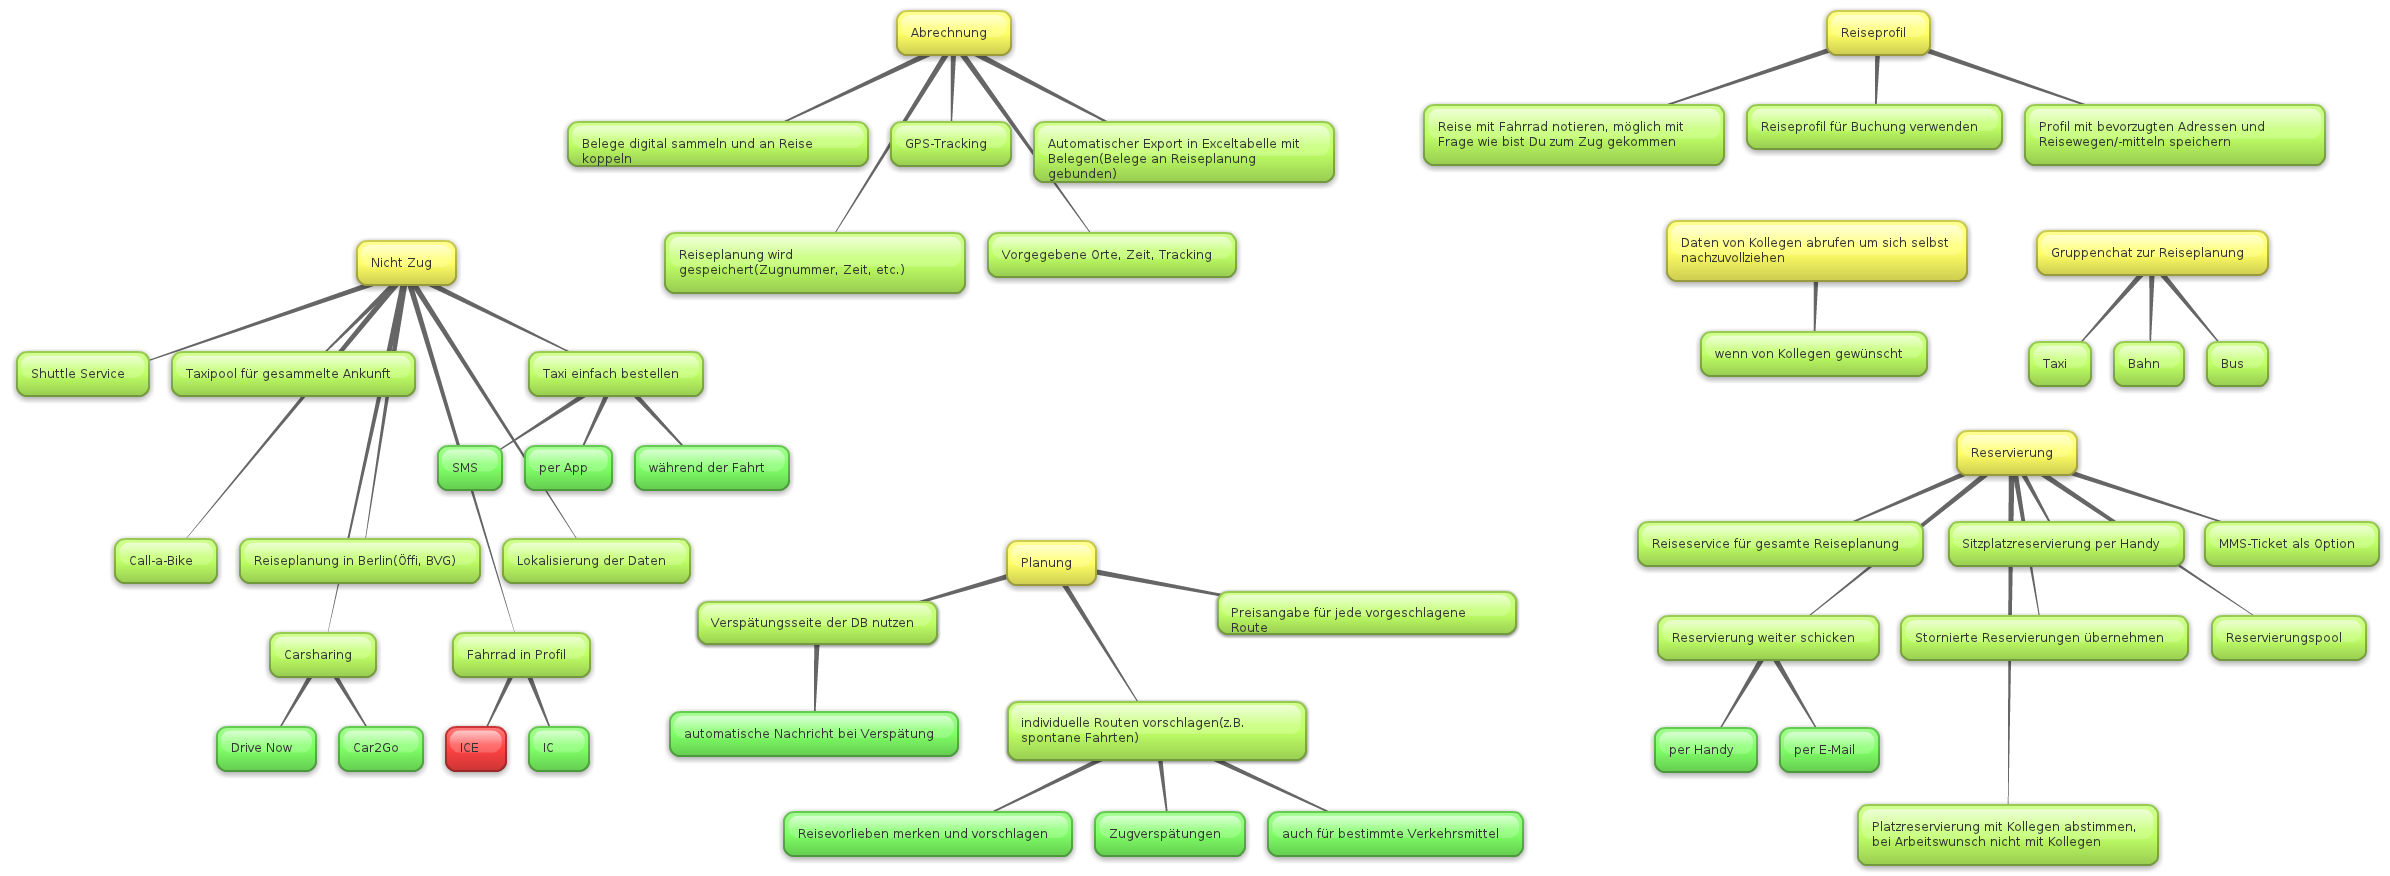
\includegraphics[width=1.0\textwidth, height=130mm]{images/konzeption.png}
\caption{conception}
\label{fig:conception}
\end{figure}
\clearpage

\section{idea 1 : taxi sharing}

In the first idea we wanted to ease the use of taxis in Wolfsburg. Often you sit  in the same train like your colleagues but you don�t know. Instead of sharing a taxi, you send more money for it and have double trouble. We wanted to create a platform where you can see who also want to take a taxi to a certain time from place A to place B. In the best case the taxi-order should be automated, so you have no stress getting your taxi punctual with no stress of searching and running(like its usually at the main line).

\section{idea 2: travel diary}

This solution should ease the payoff f the CARMEQ-workers. The application would track the position of the user and with the help of these tracks the application can calculate when the user have been traveled. At the end of each month you can use this diary to complete your own notes.


\section{decision}
 Both idea were accepted good, so its was up on us, to decide. We choose the first idea. The only reason for this decision was more interests in this theme.
 
 